\chapter{Problem Analysis and Modeling}

This chapter bridges the problem landscape articulated in Chapter~1 and the research foundations established in Chapter~2 with concrete system specifications and models. It presents a detailed analysis of requirements, functional and non-functional specifications, and comprehensive system models---use cases, UML class diagrams, sequence diagrams, activity diagrams, and state machines---that collectively define what \projectname{} must achieve and how its components interact. The modelling approach follows standard software engineering practices, ensuring that requirements are comprehensive, testable, and verifiable. Models serve dual purposes: (1) communicating system intent to stakeholders and team members, and (2) providing a blueprint for implementation in Chapter~5.

\section{Existing System and Its Problems}

The current landscape of self-directed learning systems, particularly for technical skill acquisition in resource-constrained environments like Ethiopia, is dominated by a mix of free online resources, static roadmaps, massive open online courses (MOOCs), spaced repetition tools, and emerging large language model (LLM)-based tutors. Platforms such as Khan Academy, roadmap.sh, Coursera/Udemy, Anki, and pure LLM tutoring (e.g., ChatGPT, Claude) represent the primary existing systems. While these have democratized access to knowledge, they exhibit systemic limitations rooted in design philosophies that prioritise scalability and content volume over personalisation, retention, and adaptive feedback. This section provides a detailed examination of these systems, identifying their limitations, underlying causes, affected stakeholders, and impacts.

\subsection*{Overview of Existing Systems}

Existing systems can be broadly categorised into three types:

\begin{enumerate}
    \item \textbf{Curated Content Platforms:} Platforms such as Khan Academy, Coursera, and Udemy provide structured video content and assessments, but follow a fixed, one-size-fits-all curriculum that does not adapt to individual learner progress or prior knowledge. These systems leverage free resources like YouTube tutorials, blog posts (e.g., GeeksForGeeks), and documentation (e.g., MDN Web Docs), but their aggregation and delivery mechanisms often exacerbate fragmentation rather than resolve it.
    \item \textbf{Static Roadmap Tools:} Resources like \texttt{roadmap.sh} offer visual dependency graphs of skills but lack interactivity, progress tracking, or assessment capabilities. They present a fixed, linear sequence without performance-driven progression gates.
    \item \textbf{Retention and AI Tools:} Tools such as Anki (spaced repetition flashcards) and conversational AI tutors (ChatGPT, Claude) address isolated aspects of learning but are not integrated into a coherent, mastery-based progression system.
\end{enumerate}

\subsection*{Limitations and Underlying Causes}

The limitations stem from architectural, pedagogical, and economic constraints, leading to inefficiencies in learner progression and retention.

\begin{enumerate}
    \item \textbf{Fragmentation and Lack of Coherent Structure (Tutorial Hell Phenomenon):} Most systems rely on passive, non-sequenced content delivery. YouTube recommendations and roadmap.sh provide disjointed resources without enforcing prerequisites or logical progression, caused by algorithmic biases favouring engagement metrics over pedagogical soundness. Cognitive load theory~\cite{sweller1988} explains how unstructured information overwhelms working memory, leading to reduced retention. \textbf{92\% of surveyed learners} reported difficulty finding coherent paths, highlighting how ad-hoc navigation creates knowledge gaps (e.g., jumping from HTML to React without JavaScript fundamentals).

    \item \textbf{Absence of Adaptive Feedback and Personalization:} Platforms like Khan Academy and Coursera use fixed sequences without runtime adaptation to learner performance or preferences. Pure LLM tutors hallucinate responses due to unverified knowledge bases, while Anki requires manual card creation. Self-determination theory~\cite{deci1985} shows that lack of agency reduces motivation. \textbf{85\% of learners} reported insufficient feedback, leading to false mastery (e.g., marking topics \enquote{complete} without competence verification). This results in high dropout rates (\textbf{70\%+ on Coursera}).

    \item \textbf{No Mastery-Based Progression Gates and Retention Mechanisms:} Systems like roadmap.sh lack quizzes or gates, relying on self-assessment, while Anki isolates repetition from curriculum context. Ebbinghaus's Forgetting Curve~\cite{ebbinghaus1885} is ignored, causing skill decay over time---\textbf{78\% of learners forget concepts after 14 days} without review. Mastery learning principles~\cite{bloom1968} advocate competence-based gates, yet existing tools lead to downstream failures. In resource-constrained contexts, this amplifies economic barriers, as learners cannot afford premium alternatives.

    \item \textbf{Quality Variability and Resource Overload:} Algorithmic curation (e.g., LinkedIn Learning) prioritises popularity over accuracy, leading to unreliable content. Manual curation (Khan Academy) is resource-intensive, limiting coverage to established domains. This creates cognitive overload as learners sift through mixed-quality sources. Focus groups revealed biases toward entertainment-oriented content, misaligning with deep learning needs.
\end{enumerate}

\subsection*{Stakeholders and Impacts}

The stakeholders affected by these limitations are:

\begin{itemize}
    \item \textbf{Primary Stakeholders---Learners (Ethiopian Students, Junior Developers, Career-Changers):} Frustration from \enquote{tutorial hell} leads to demotivation, skill gaps, and delayed career progression. In Ethiopia, where premium mentorship is prohibitive, this perpetuates economic inequality---learners waste time (85\% report inefficient paths), experience high dropout, and face retention decay, hindering employability in tech sectors.
    \item \textbf{Secondary Stakeholders---Educators and Institutions (e.g., AASTU Faculty):} Overburdened with remedial teaching due to self-directed gaps; limited tools for integrating adaptive systems into curricula, reducing institutional efficacy.
    \item \textbf{Tertiary Stakeholders---Content Providers and Communities (e.g., FreeCodeCamp, Reddit):} Underutilised high-quality resources due to discovery barriers; community biases amplify unreliable content, eroding trust.
\end{itemize}

\textbf{Overall Impact:} These limitations create a vicious cycle: fragmentation increases cognitive load, lack of feedback fosters false confidence, and decay causes repeated failures, impacting motivation and long-term skill acquisition. In developing economies, this widens the digital divide, as learners cannot compete with those in resource-rich environments.

\subsection*{Utilization of Analytical Tools and Techniques}

To understand the complexity of the problem, the following analytical tools and techniques were employed:

\begin{itemize}
    \item \textbf{Stakeholder Engagement:} Semi-structured interviews with domain experts (n=5) and learner surveys (n=30) quantified pain points, including the 78\% skill decay rate, 92\% path fragmentation, and 85\% insufficient feedback.
    \item \textbf{Competitive Gap Analysis:} Synthesised via a landscape comparison table mapping strengths and gaps of existing solutions against \projectname{} innovations.
    \item \textbf{Cognitive and Pedagogical Frameworks:} Applied theories (Forgetting Curve, Mastery Learning, Cognitive Load Theory, Self-Determination Theory) to model impacts and validate proposed solutions.
    \item \textbf{Prototyping and Simulation:} Early wireframes and decay algorithm prototypes validated assumptions about learner progression and retention mechanics.
\end{itemize}

\section{Requirements Elicitation and Specification}

\subsection*{Elicitation Methodology}

Requirements were gathered through multi-stakeholder engagement:

\begin{enumerate}
    \item \textbf{Domain Expert Interviews:} Semi-structured interviews with five software engineering educators, industry practitioners, and experienced self-taught engineers were conducted to understand learning challenges, effective pedagogical strategies, and domain-specific sequencing principles. Key insights included: learners struggle with unstructured, non-sequential content; assessment-driven progression increases motivation; resource modality (documentation vs.\ tutorial) significantly affects learning outcomes.
    \item \textbf{Learner Surveys and Feedback Sessions:} An online survey (30 respondents: Ethiopian students, junior developers, career-changers) identified pain points: tutorial fragmentation (92\% reported difficulty finding coherent learning paths), lack of feedback (85\% noted insufficient guidance on mastery), and skill decay (78\% forgot concepts after weeks of non-practice). Focus group discussions (two sessions, 15 participants) validated proposed solutions and identified usability priorities.
    \item \textbf{Competitive Analysis:} Analysis of existing platforms (Khan Academy, roadmap.sh, Coursera, Anki, ChatGPT tutoring) identified gaps and best practices, informing feature prioritisation and differentiation.
\end{enumerate}

\subsection*{Functional Requirements}

Functional requirements specify what the system must do, organised by use case and subsystem:

\begin{enumerate}
    \item[\textbf{FR1:}] \textbf{Ontology Management}
        \begin{enumerate}
            \item[\textbf{FR1.1:}] The system shall generate a learning ontology (DAG of learning nodes) for a given domain using the Teacher Model (offline LLM), producing a JSON structure with node identifiers, learning outcomes, prerequisites, and estimated effort.
            \item[\textbf{FR1.2:}] The system shall support expert verification workflows, enabling domain experts to review generated ontologies, flag errors, and approve for production deployment.
            \item[\textbf{FR1.3:}] The system shall persist and version ontologies, maintaining a history of changes and enabling rollback if necessary.
        \end{enumerate}

    \item[\textbf{FR2:}] \textbf{Learner Management}
        \begin{enumerate}
            \item[\textbf{FR2.1:}] The system shall enable user registration (email, social login via Google/GitHub) and profile creation.
            \item[\textbf{FR2.2:}] The system shall track learner progress, including node completion status, quiz scores, attempts, and timestamps.
            \item[\textbf{FR2.3:}] The system shall compute and display learner statistics (total nodes completed, average quiz score, time spent, learning pace).
        \end{enumerate}

    \item[\textbf{FR3:}] \textbf{Quiz Generation and Delivery}
        \begin{enumerate}
            \item[\textbf{FR3.1:}] The system shall generate domain-specific quizzes using the Tutor Model (runtime LLM), producing 3--5 questions per node, grounded in the node's learning outcomes.
            \item[\textbf{FR3.2:}] The system shall support multiple question types: multiple-choice, short-answer, code-completion, true-false, matching.
            \item[\textbf{FR3.3:}] The system shall evaluate quiz responses, compute scores, and provide immediate feedback on correctness.
            \item[\textbf{FR3.4:}] The system shall generate micro-quizzes (2--3 questions) triggered by Mastery Decay transitions.
        \end{enumerate}

    \item[\textbf{FR4:}] \textbf{Gatekeeper Pattern Implementation}
        \begin{enumerate}
            \item[\textbf{FR4.1:}] The system shall enforce three-tier progression logic: Pass (\(\ge 80\%\) $\rightarrow$ unlock next node + challenge project), Marginal Pass (70--79\% $\rightarrow$ unlock but flag for review), Fail (\(<70\%\) $\rightarrow$ lock and trigger remediation).
            \item[\textbf{FR4.2:}] The system shall validate prerequisites before unlocking nodes, preventing progression if prerequisites are not mastered.
            \item[\textbf{FR4.3:}] Upon Pass (\(\ge 80\%\)), the system shall recommend a challenge project relevant to the node's outcomes.
            \item[\textbf{FR4.4:}] Upon Fail (\(<70\%\)), the system shall trigger resource adaptation or prerequisite review based on failure severity.
        \end{enumerate}

    \item[\textbf{FR5:}] \textbf{Resource Recommendation and Curation}
        \begin{enumerate}
            \item[\textbf{FR5.1:}] The system shall integrate the Google Programmable Search Engine (PSE) API to fetch resource links from pre-approved whitelisted domains.
            \item[\textbf{FR5.2:}] The system shall validate recommended links via automated checks (HTTP status, content freshness, relevance).
            \item[\textbf{FR5.3:}] The system shall support learner feedback on resource quality (rating, comments) and use ratings to inform future recommendations.
            \item[\textbf{FR5.4:}] Upon resource adaptation (triggered by Gatekeeper Fail), the system shall recommend alternative resources with different modalities (e.g., swap documentation for tutorial).
        \end{enumerate}

    \item[\textbf{FR6:}] \textbf{Mastery Decay and Spaced Repetition}
        \begin{enumerate}
            \item[\textbf{FR6.1:}] The system shall track the time since a node was last reviewed and compute decay state (Green $\le 14$ days, Yellow $14$--$30$ days, Red $>30$ days).
            \item[\textbf{FR6.2:}] Upon transition to Yellow or Red, the system shall automatically generate and present a micro-quiz to the learner.
            \item[\textbf{FR6.3:}] The system shall visualise decay states in the learner's roadmap (colour-coded nodes).
            \item[\textbf{FR6.4:}] The system shall send notifications (in-app or email) alerting learners to nodes requiring review.
        \end{enumerate}

    \item[\textbf{FR7:}] \textbf{Multi-Path Branching}
        \begin{enumerate}
            \item[\textbf{FR7.1:}] The system shall identify branching points in the ontology where learners can choose alternative paths (e.g., Frontend vs.\ Backend).
            \item[\textbf{FR7.2:}] Upon reaching a branching point, the system shall present a choice question and path recommendations.
            \item[\textbf{FR7.3:}] After learner selection, the system shall dynamically adjust the roadmap to display the selected path and its prerequisites.
            \item[\textbf{FR7.4:}] The system shall ensure paths reconverge at advanced nodes, maintaining semantic coherence.
        \end{enumerate}

    \item[\textbf{FR8:}] \textbf{User Interfaces}
        \begin{enumerate}
            \item[\textbf{FR8.1:}] The web interface (React) shall display the ontology as an interactive DAG visualisation with zoom, pan, and filtering capabilities.
            \item[\textbf{FR8.2:}] The web interface shall include quiz delivery UI, progress dashboard, resource panel, and learner settings.
            \item[\textbf{FR8.3:}] The mobile interface (Flutter) shall provide touch-optimized navigation, offline support (cached roadmap data), and push notifications.
            \item[\textbf{FR8.4:}] Both interfaces shall be responsive, adapting to different screen sizes (mobile, tablet, desktop).
        \end{enumerate}
\end{enumerate}

\subsection*{Non-Functional Requirements}

Non-functional requirements specify quality attributes and constraints:

\begin{enumerate}
    \item[\textbf{NFR1:}] \textbf{Performance}
        \begin{enumerate}
            \item[\textbf{NFR1.1:}] Page load time for roadmap visualisation shall not exceed 2 seconds on typical internet connections (\(>5\) Mbps).
            \item[\textbf{NFR1.2:}] API response time for quiz delivery and scoring shall not exceed 500 milliseconds (p95).
            \item[\textbf{NFR1.3:}] LLM-based quiz generation shall complete within 3 seconds of user request, leveraging caching to accelerate repeated requests.
        \end{enumerate}

    \item[\textbf{NFR2:}] \textbf{Scalability}
        \begin{enumerate}
            \item[\textbf{NFR2.1:}] The system shall support 1,000 concurrent users without degradation in performance (load testing baseline).
            \item[\textbf{NFR2.2:}] Database and cache layers shall scale horizontally (read replicas, sharding) to support 10,000+ daily active users.
            \item[\textbf{NFR2.3:}] The system shall support efficient multi-tenancy (future feature), enabling independent deployments per institution or community.
        \end{enumerate}

    \item[\textbf{NFR3:}] \textbf{Availability and Reliability}
        \begin{enumerate}
            \item[\textbf{NFR3.1:}] System uptime shall be \(\ge 99.5\%\) (measured monthly).
            \item[\textbf{NFR3.2:}] Critical data (learner progress, quiz responses) shall be backed up daily, with recovery capability within 4 hours.
            \item[\textbf{NFR3.3:}] The system shall implement graceful degradation: if LLM API is unavailable, fallback to pre-generated quizzes and explanations.
        \end{enumerate}

    \item[\textbf{NFR4:}] \textbf{Security}
        \begin{enumerate}
            \item[\textbf{NFR4.1:}] User authentication shall use JWT tokens with secure token storage (httpOnly cookies).
            \item[\textbf{NFR4.2:}] Sensitive data (user profiles, quiz responses) shall be encrypted in transit (HTTPS) and at rest (database encryption).
            \item[\textbf{NFR4.3:}] The system shall implement role-based access control (RBAC): learner, instructor, admin, system administrator roles with distinct permissions.
            \item[\textbf{NFR4.4:}] The system shall sanitize user inputs and API responses to prevent SQL injection and XSS attacks.
            \item[\textbf{NFR4.5:}] Learner data shall be treated as confidential; no personal data shall be shared with third-party services without explicit consent.
        \end{enumerate}

    \item[\textbf{NFR5:}] \textbf{Usability}
        \begin{enumerate}
            \item[\textbf{NFR5.1:}] Learners shall complete onboarding (account creation, path selection) in \(<5\) minutes.
            \item[\textbf{NFR5.2:}] Quiz interface shall be intuitive, with clear instructions and immediate feedback.
            \item[\textbf{NFR5.3:}] Roadmap visualisation shall be interpretable by non-technical learners, with intuitive legend and help tooltips.
            \item[\textbf{NFR5.4:}] System error messages shall be clear and actionable, guiding learners toward resolution.
        \end{enumerate}

    \item[\textbf{NFR6:}] \textbf{Maintainability and Extensibility}
        \begin{enumerate}
            \item[\textbf{NFR6.1:}] Code shall follow established standards (JavaScript/TypeScript style guides, REST API conventions) and include comprehensive documentation.
            \item[\textbf{NFR6.2:}] The system architecture shall enable addition of new domains without redesigning core components.
            \item[\textbf{NFR6.3:}] API endpoints shall be versioned (v1, v2) to support backward compatibility during upgrades.
        \end{enumerate}

    \item[\textbf{NFR7:}] \textbf{Localization and Cultural Adaptation}
        \begin{enumerate}
            \item[\textbf{NFR7.1:}] The UI shall support Amharic, English, and Oromo languages initially, with extensibility to other Ethiopian languages.
            \item[\textbf{NFR7.2:}] Content and examples shall reflect Ethiopian context (e.g., local tech companies, Ethiopian learner profiles, culturally appropriate imagery).
            \item[\textbf{NFR7.3:}] The system shall work reliably on low-bandwidth networks (\(<2\) Mbps), common in rural Ethiopia.
        \end{enumerate}
\end{enumerate}

\section{System Modeling}

\subsection{Use Case Model}

Use cases capture interactions between actors (users) and the system. Table~\ref{tab:ch03_usecases} presents the primary use cases identified for \projectname{}, covering the interactions of learners, domain experts, and administrators with the system.

\begin{table}[htbp]
    \centering
    \caption{Primary Use Cases}
    \label{tab:ch03_usecases}
    \small
    \begin{tabular}{@{}p{2cm}p{1.8cm}p{2.5cm}p{5.5cm}p{2.7cm}@{}}
        \toprule
        \textbf{Use Case} & \textbf{Primary Actor} & \textbf{Preconditions} & \textbf{Main Flow} & \textbf{Postconditions} \\
        \midrule
        UC1: Browse Roadmap & Learner & Logged in, ontology loaded & 1. Display DAG visualisation 2. Learner explores nodes 3. System shows details, learning outcomes, prerequisites & Learner understands path and requirements \\
        UC2: Attempt Quiz & Learner & Node unlocked, learner selected Take Quiz & 1. Generate quiz (3--5 questions) 2. Learner answers 3. Evaluate responses, compute score & Score recorded; Gatekeeper triggered \\
        UC3: Resource Recommendation & Learner & Quiz failed (\(<70\%\)), adaptation triggered & 1. Identify adapted resources 2. Present 3--5 links with descriptions 3. Learner selects resources & Alternative materials accessed \\
        UC4: Spaced Repetition Reminder & Learner & Node in Yellow/Red decay state & 1. Generate micro-quiz notification 2. Present micro-quiz (2--3 questions) 3. Learner attempts, system scores & Decay state updated; learner re-engaged \\
        UC5: Select Learning Path & Learner & Reached branching point & 1. Present choice question and descriptions 2. Learner selects path 3. Update roadmap with selected path nodes & Roadmap personalised \\
        UC6: Verify Ontology & Domain Expert & Ontology generated by Teacher Model & 1. Expert reviews nodes, prerequisites, outcomes 2. Marks correct or flags for revision 3. Aggregates feedback, expert confirms & Verified ontology deployed \\
        UC7: Manage Domain Whitelist & Admin/Domain Curator & Need to update trusted providers & 1. View current whitelist (e.g., MDN) 2. Add/remove domains 3. System applies to PSE API queries & Resources restricted to approved \\
        UC8: View Progress Dashboard & Learner & Logged in & 1. Display statistics (nodes completed, avg score, time) 2. Show decay state visualisation (Green/Yellow/Red) 3. Filter by domain or time & Visibility into learning progress \\
        \bottomrule
    \end{tabular}
\end{table}

\subsection{Functional Requirements Traceability}

Table~\ref{tab:ch03_traceability} maps each use case to the functional requirements it realises, ensuring comprehensive coverage and providing a basis for validation.

\begin{table}[htbp]
    \centering
    \caption{Use Case to Functional Requirement Mapping}
    \label{tab:ch03_traceability}
    \small
    \begin{tabular}{@{}p{4.5cm}p{9.5cm}@{}}
        \toprule
        \textbf{Use Case} & \textbf{Functional Requirements} \\
        \midrule
        UC1: Browse Roadmap & FR1.1, FR1.3, FR8.1 \\
        UC2: Attempt Quiz & FR3.1, FR3.2, FR3.3, FR4.1, FR4.2 \\
        UC3: Receive Resource Recommendation & FR5.1, FR5.2, FR5.4, FR4.4 \\
        UC4: Receive Spaced Repetition Reminder & FR6.1, FR6.2, FR6.3, FR6.4 \\
        UC5: Select Learning Path & FR7.1, FR7.2, FR7.3, FR7.4 \\
        UC6: Verify Ontology & FR1.2, FR1.3 \\
        UC7: Manage Domain Whitelist & FR5.1 \\
        UC8: View Progress Dashboard & FR2.3, FR6.3 \\
        \bottomrule
    \end{tabular}
\end{table}

\subsection{UML Class Diagram}

Figure~\ref{fig:ch03_classdiagram} presents the core domain model of \projectname{}, illustrating the principal entities and their relationships.

\begin{figure}[H]
    \centering
    
\includegraphics[width=\textwidth]{figures/images/image11.png}
    \caption{UML Class Diagram}
    \label{fig:ch03_classdiagram}
\end{figure}

\subsection{Dynamic Models of a System}

The dynamic behaviour of \projectname{} is captured through sequence diagrams, activity diagrams, and a state machine diagram, each focusing on a critical interaction or lifecycle within the system.

\subsubsection{Sequence Diagrams}

\paragraph{Quiz Attempt and Gatekeeper Flow}\mbox{}\\

Figure~\ref{fig:ch03_quizgatekeeper} models the interaction sequence when a learner attempts a quiz, including the gatekeeper decision that determines whether the learner may proceed to dependent nodes.

\begin{figure}[H]
    \centering
    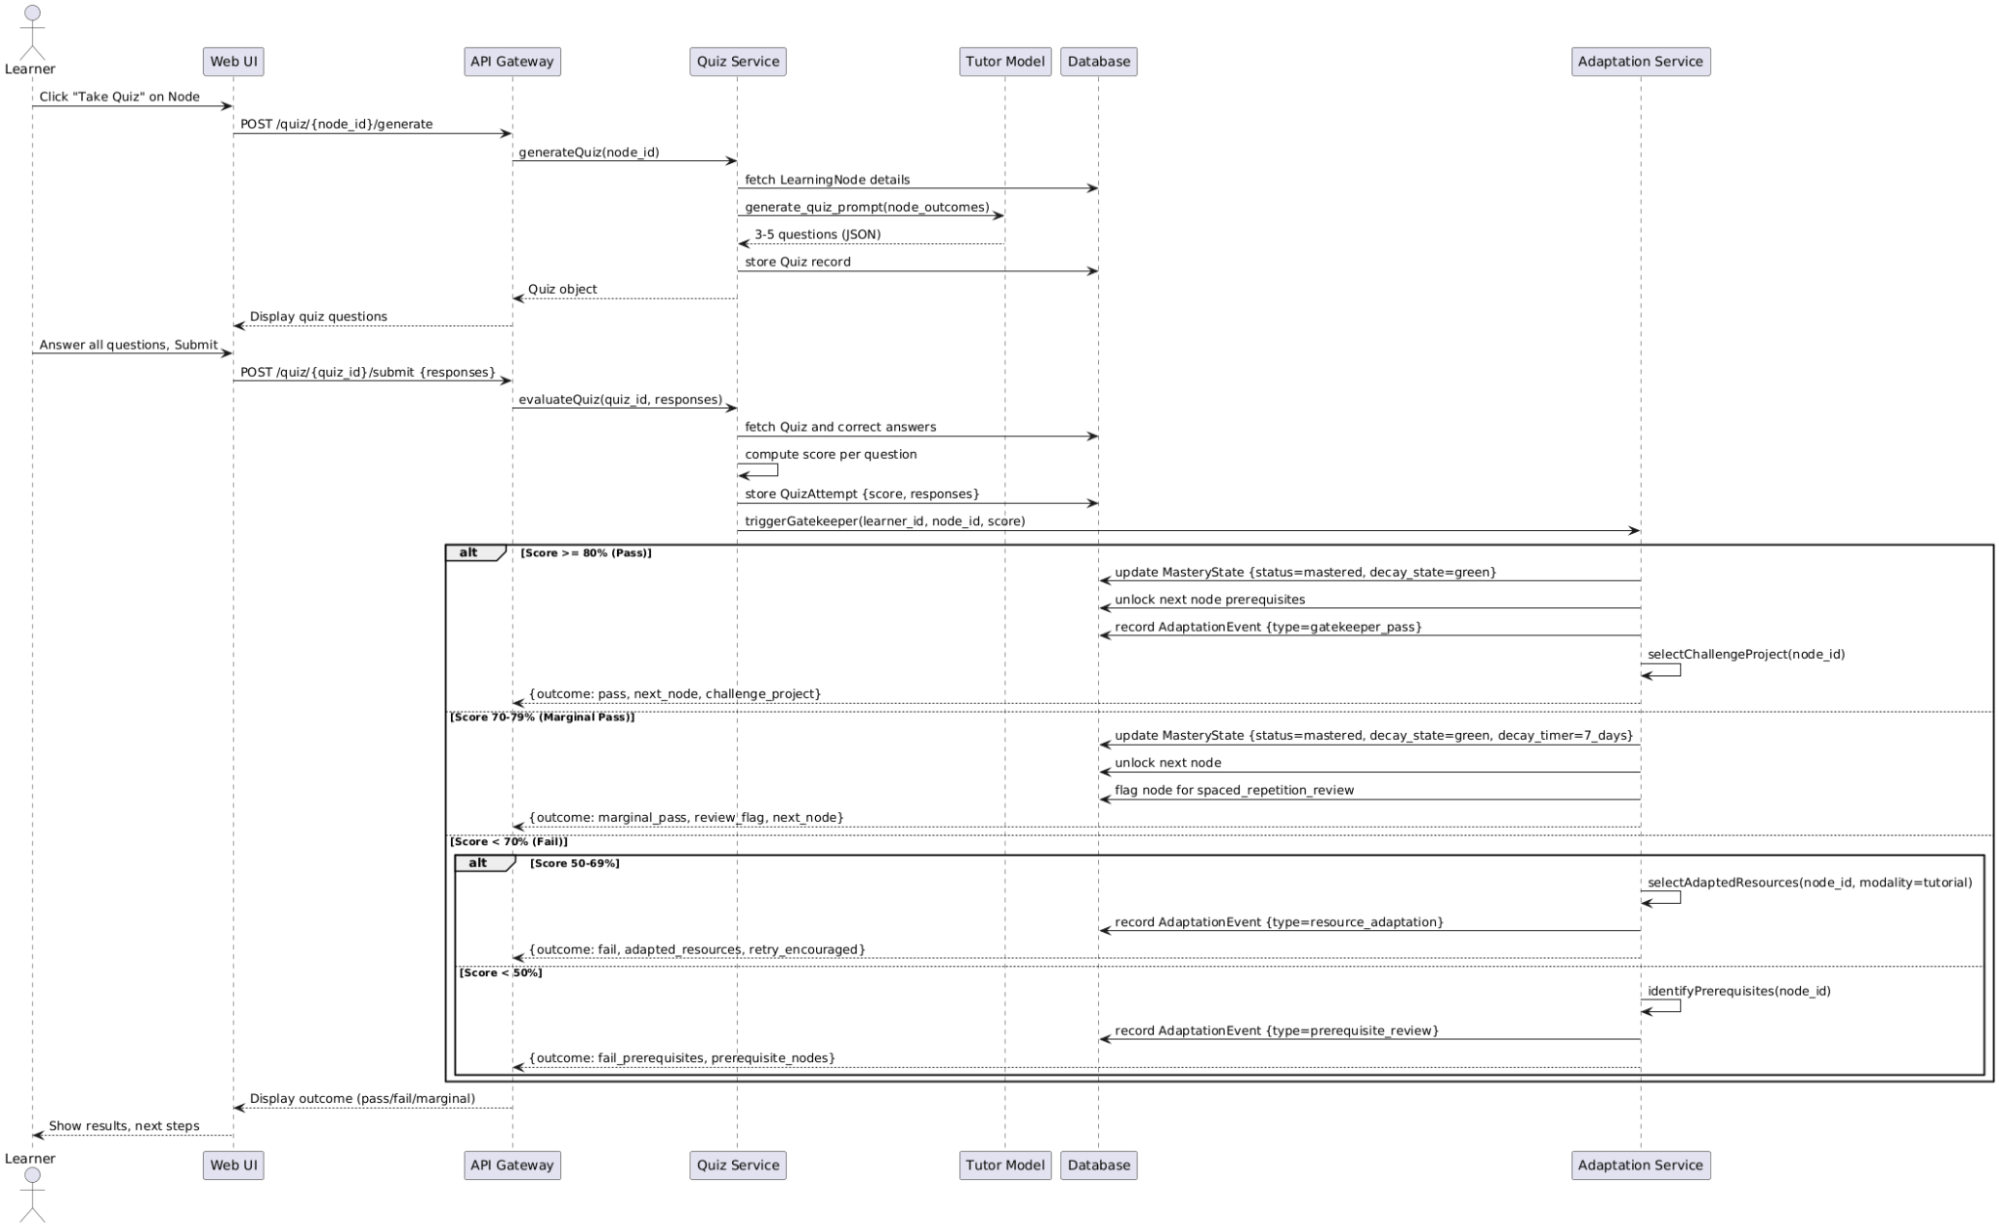
\includegraphics[width=\textwidth]{figures/images/image4.png}
    \caption{Quiz Attempt and Gatekeeper Flow}
    \label{fig:ch03_quizgatekeeper}
\end{figure}

\paragraph{Mastery Decay and Spaced Repetition Trigger}\mbox{}\\

Figure~\ref{fig:ch03_masterydecay} models the periodic decay check and the triggered spaced repetition workflow that prompts learners to reinforce fading knowledge.

\begin{figure}[H]
    \centering
    
\includegraphics[width=\textwidth]{figures/images/image5.png}
    \caption{Mastery Decay and Spaced Repetition Trigger}
    \label{fig:ch03_masterydecay}
\end{figure}

\paragraph{Multi-Path Branching Selection}\mbox{}\\

Figure~\ref{fig:ch03_multipath} illustrates the sequence of interactions when a learner encounters a branching point and selects a specialisation path.

\begin{figure}[H]
    \centering
    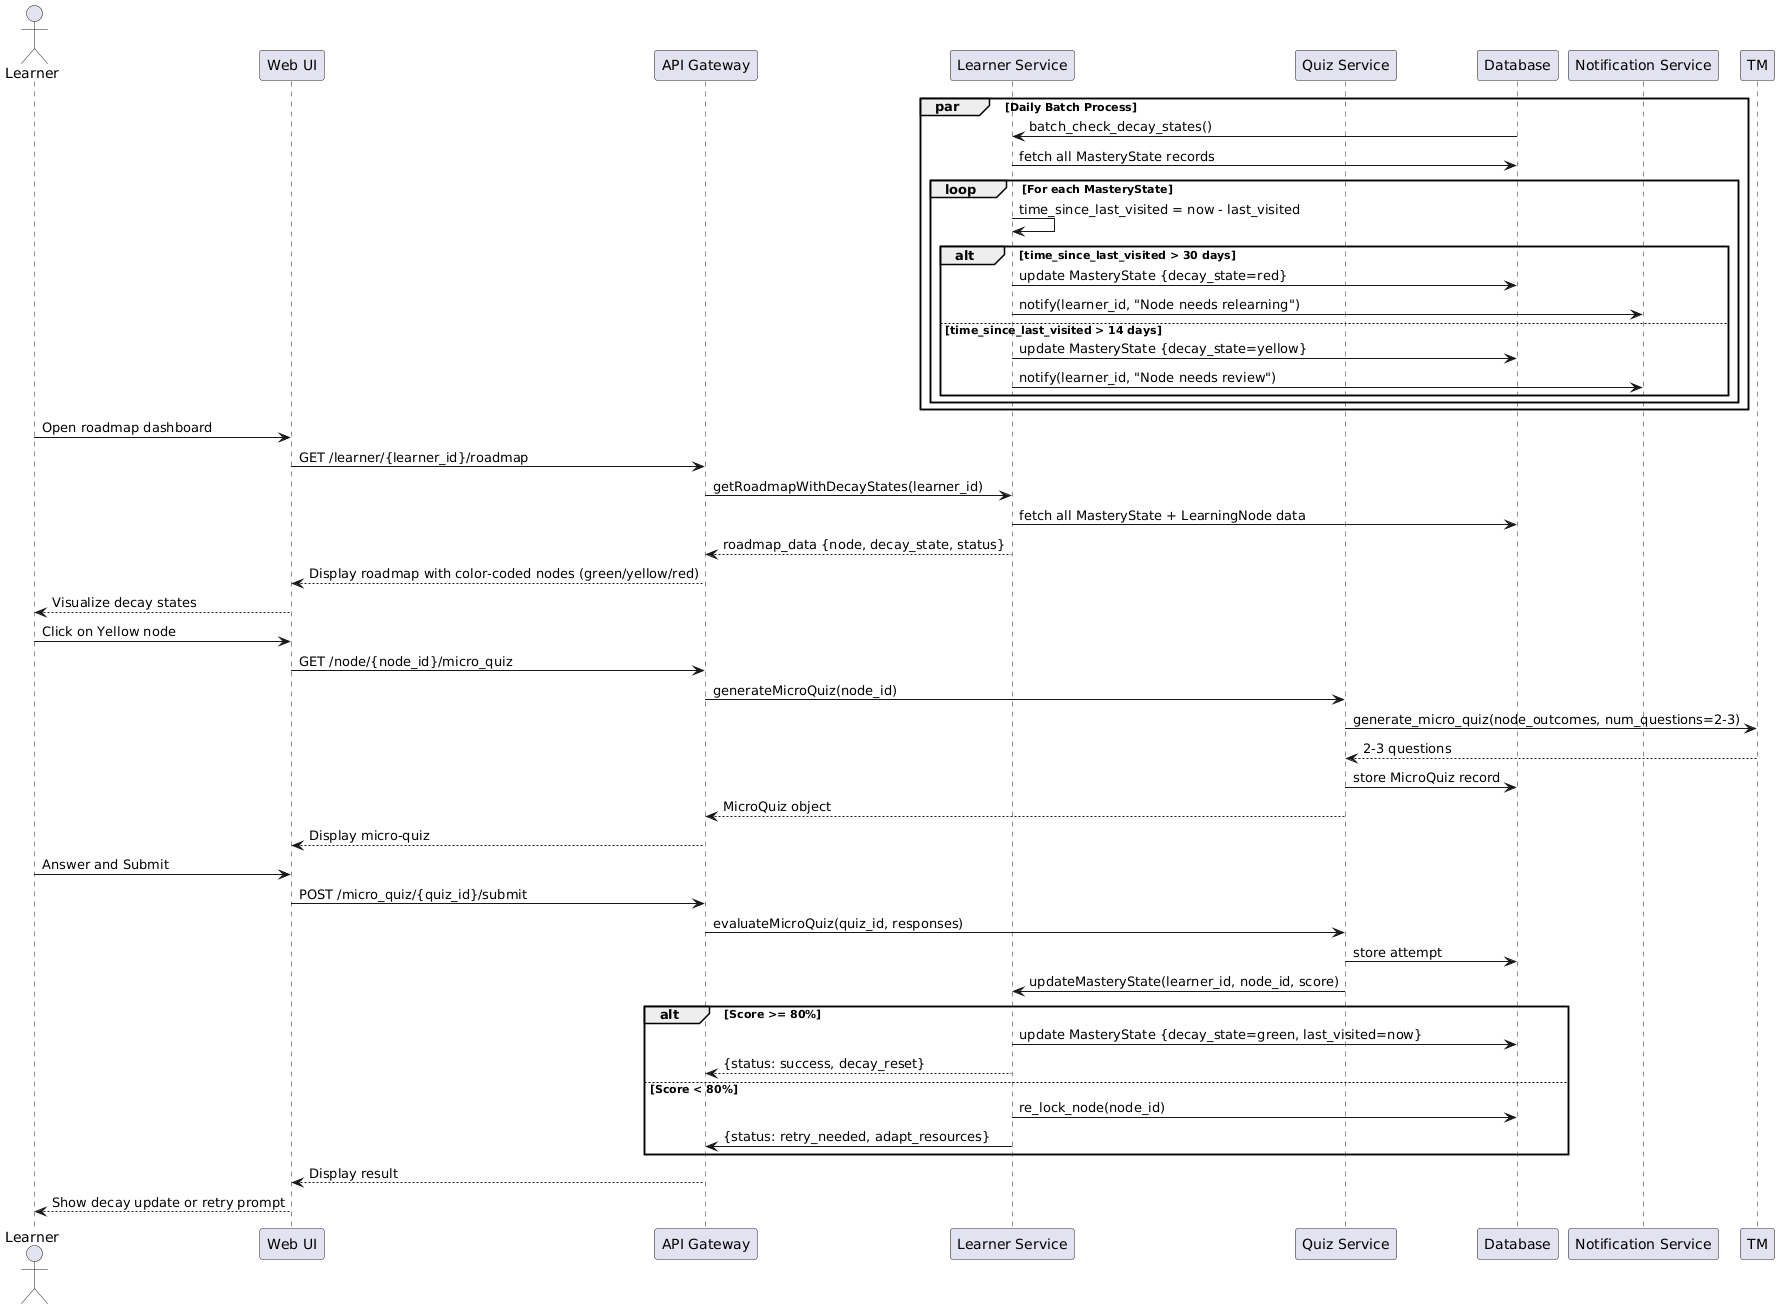
\includegraphics[width=\textwidth]{figures/images/image1.png}
    \caption{Multi-Path Branching Selection}
    \label{fig:ch03_multipath}
\end{figure}

\subsubsection{Activity Diagrams}

\paragraph{Learner Progression Activity Flow}\mbox{}\\

Figure~\ref{fig:ch03_progression} models the overall activity flow of a learner navigating through the roadmap, from node exploration through assessment and progression.

\begin{figure}[H]
    \centering
    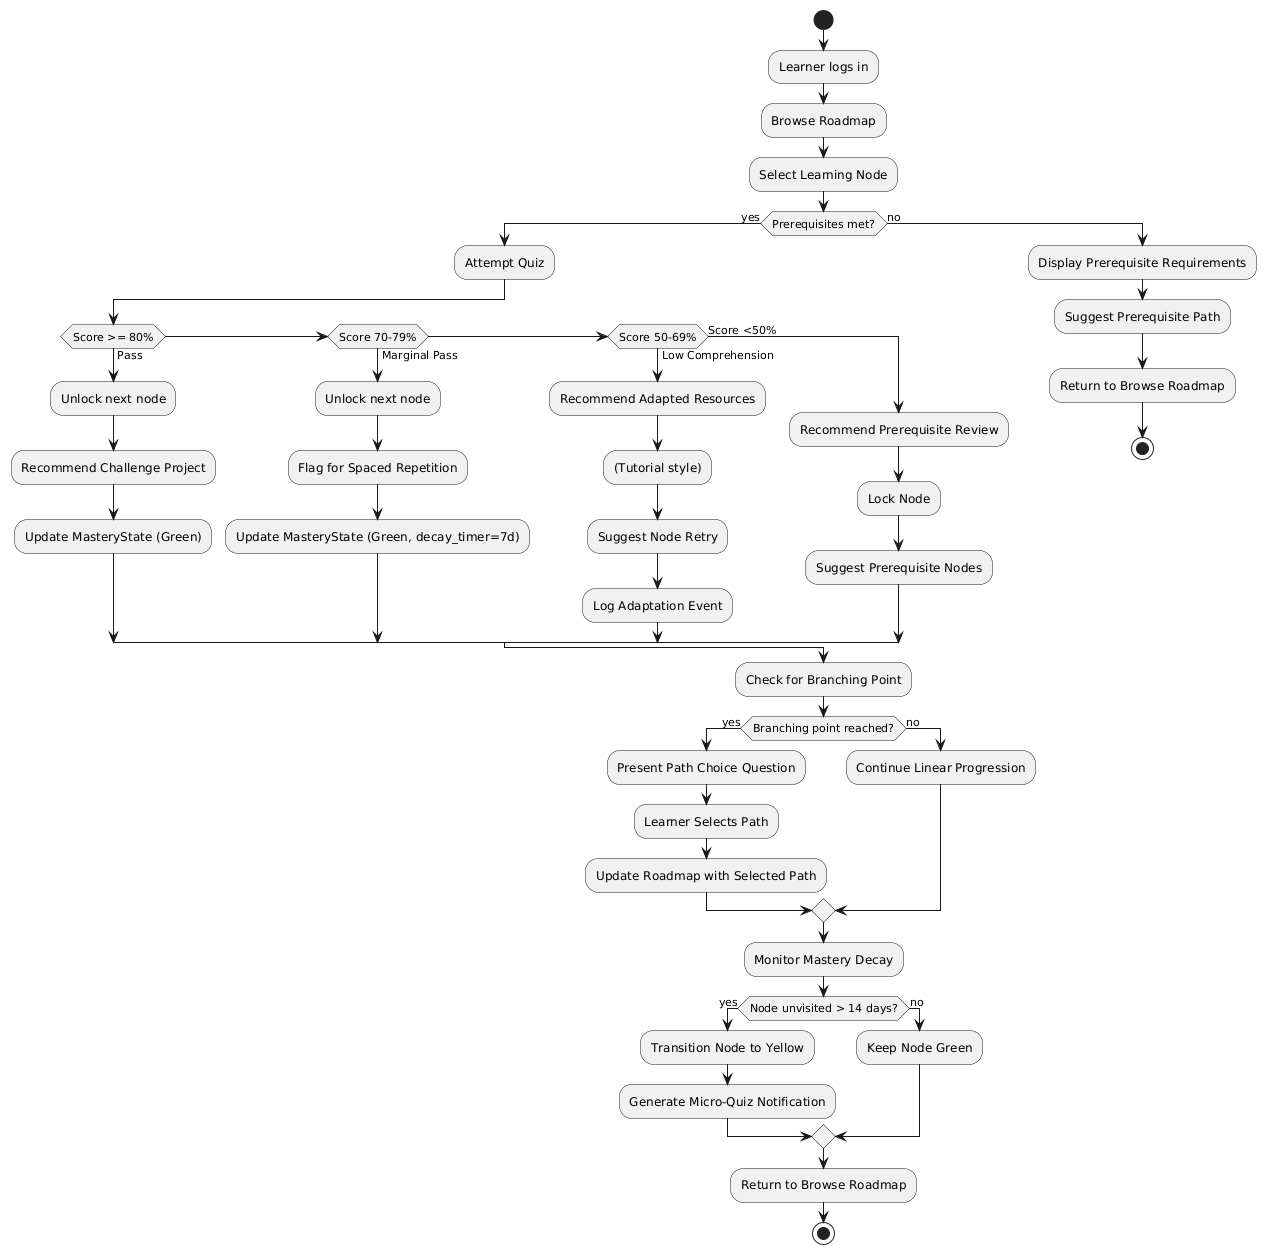
\includegraphics[width=\textwidth]{figures/images/image8.png}
    \caption{Learner Progression Activity Flow}
    \label{fig:ch03_progression}
\end{figure}

\paragraph{Gatekeeper Decision Activity}\mbox{}\\

Figure~\ref{fig:ch03_gatekeeper} details the decision logic within the gatekeeper component when evaluating quiz results and determining access to dependent nodes.

\begin{figure}[H]
    \centering
    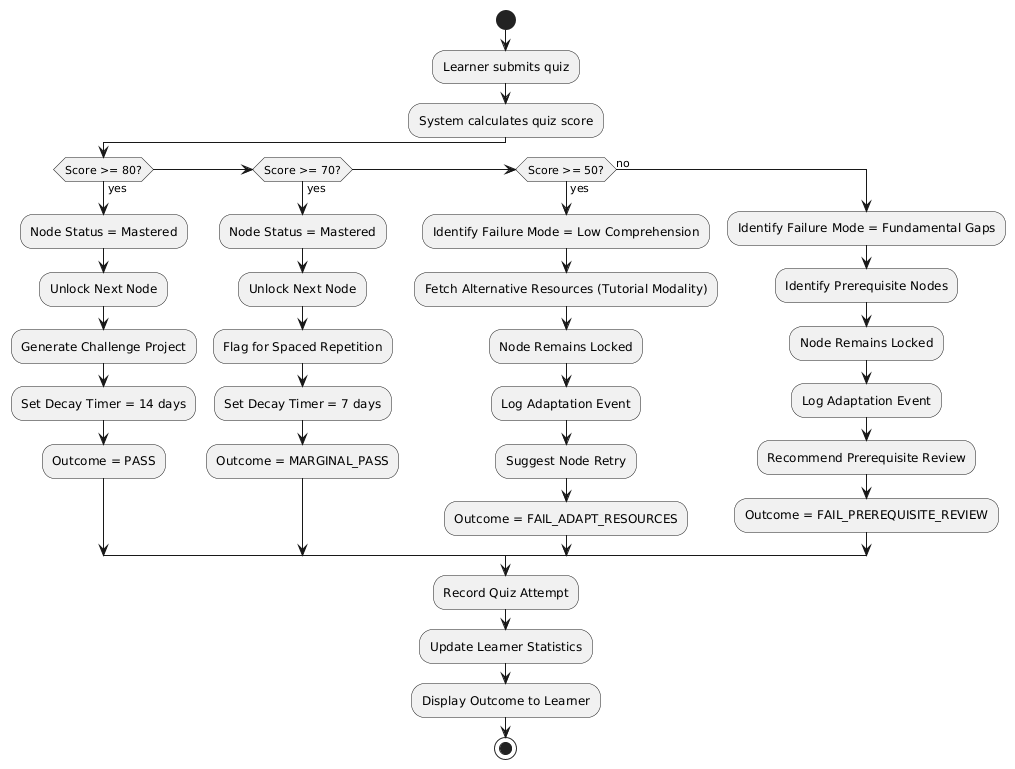
\includegraphics[width=\textwidth]{figures/images/image3.png}
    \caption{Gatekeeper Decision Activity}
    \label{fig:ch03_gatekeeper}
\end{figure}

\subsubsection{State Machine Diagram}

\paragraph{Node Mastery State Machine}\mbox{}\\

Figure~\ref{fig:ch03_statemachine} defines the mastery states (Green, Yellow, Red) that each learning node can occupy, including the transitions triggered by assessment events and the passage of time.

\begin{figure}[H]
    \centering
    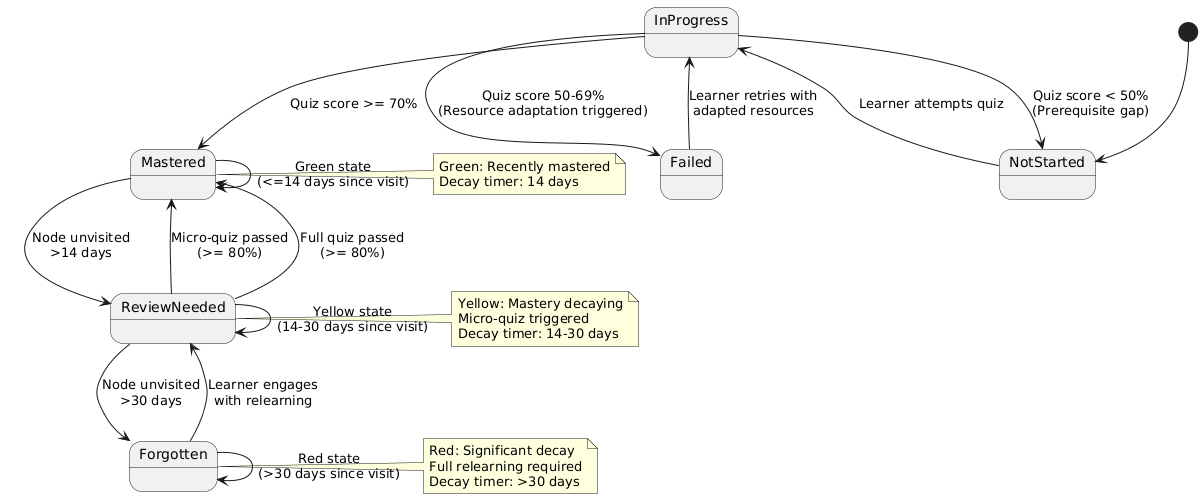
\includegraphics[width=\textwidth]{figures/images/image2.png}
    \caption{Node Mastery State Machine}
    \label{fig:ch03_statemachine}
\end{figure}

\section{Model Validation}

The requirements and models presented in this chapter were validated through the following approaches:

\begin{enumerate}
    \item \textbf{Requirements Review with Stakeholders:} The functional and non-functional requirements were reviewed with the five domain expert interviewees and a subset of survey respondents. Domain experts, learners, and team members reviewed requirements specifications, ensuring completeness and feasibility. Feedback led to refinements in the gatekeeper threshold and the addition of the multi-path branching requirements (FR7).

    \item \textbf{Traceability Analysis:} Each functional requirement was mapped to at least one use case (Table~\ref{tab:ch03_traceability}), and each use case was linked back to stakeholder needs identified during elicitation. Functional requirements are traced to use cases, and use cases are traced back to problems (Chapter~1) and research foundations (Chapter~2), ensuring all requirements are justified. This bidirectional traceability ensures that no requirement is orphaned and that every use case is justified by an underlying stakeholder concern.

    \item \textbf{Testability Assessment:} Each requirement was reviewed for testability: is there a measurable criterion for success? Non-testable requirements were refined. For example, \enquote{Quiz interface shall be intuitive} is too vague; it is refined to \enquote{Quiz interface shall support task completion by 95\% of users within 2 minutes on first attempt} (testable). Each functional requirement was evaluated for testability by defining measurable acceptance criteria.

    \item \textbf{Feasibility and Risk Analysis:} Requirements were assessed for technical feasibility within scope and budget. High-risk requirements (e.g., real-time LLM generation under load) were flagged and mitigation strategies identified (caching, fallbacks, pre-generation). Key risks identified include LLM API latency for FR3.1 (quiz generation), mitigated by the 3-second threshold in NFR1, and the complexity of maintaining the ontology DAG for large domains, mitigated by the modular ontology management interface in FR1.
\end{enumerate}

Overall, the validation confirms that the specified requirements are complete, consistent, testable, and achievable within the project scope.
